\subsection{Create the DSL Projects}

Let's start creating the projects for the Questionniare DSL. Open the New
Project Wizard with \emph{File / New / Project}. Choose ``Xtext Project'' and press
``Next''.

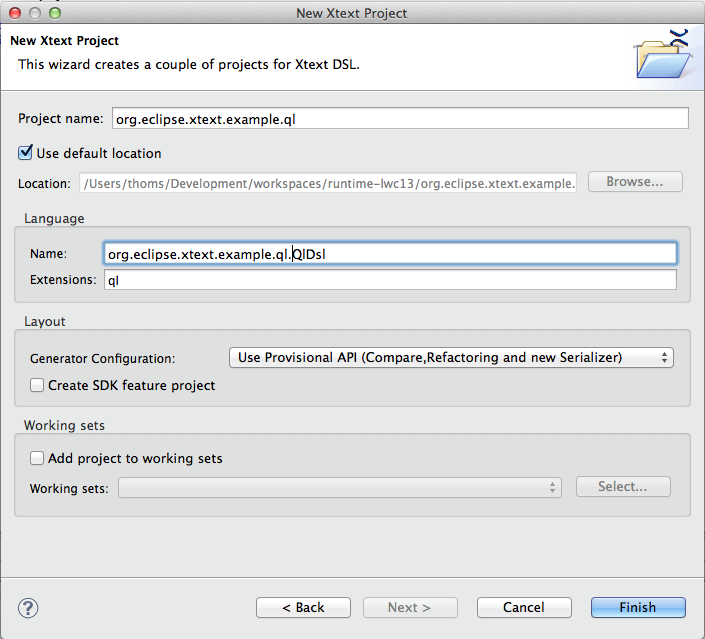
\includegraphics[width=17cm]{./images/chapter01/NewXtextProjectWizard.png}

On the project wizard page enter:
\begin{enumerate}
  \item Project name: \texttt{org.eclipse.xtext.example.ql}. Xtext will create
  multiple projects, which share this prefix. It is a convention to use
  a lowercase, dot-separated name.
  \item Language name: \texttt{org.eclipse.xtext.example.ql.QlDsl}. This is an
  identifier for the language, which must be unique and follows a Java
  full qualified identifier name pattern.
  \item Language Extensions: \texttt{ql}. This will be the file extension for
  DSL files.
  \item Uncheck the option ``Create SDK feature project''. It would not harm to
  have that checked, it would just create an additional
  \href{http://www.vogella.com/articles/EclipseFeatureProject/article.html}{Feature
  Project}, which we do not handle in this tutorial any further.
\end{enumerate}

Now press ``Finish''. Xtext will generate for you 3 projects into your workspace:

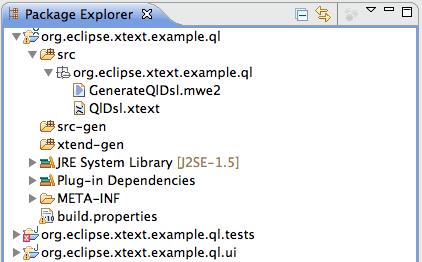
\includegraphics{./images/chapter01/WorkspaceAfterWizard.png}

\begin{itemize}
  \item \texttt{org.eclipse.xtext.example.ql}: This is the Runtime Project,
  which holds the language definition and any implementation which is not UI
  dependent. Most of the implementation details of this tutorial will be done in
  this project.
  \item \texttt{org.eclipse.xtext.example.ql.tests}: This project is intended to
  hold test code for the language. Tests are implemented with JUnit. Xtext will
  generate some infrastructure code required for tests into here. We won't deal
  testing of DSLs in this tutorial any further. You can close or remove this
  project if you want.
  \item \texttt{org.eclipse.xtext.example.ql.ui}: Xtext produces a language
  specific text editor. The editor is an Eclipse plugin. While the runtime part
  of the language could be used in any UI or even from command-line, the Editor
  is dependent on the Eclipse platform.
\end{itemize}

All projects are almost empty right now. Only the Runtime Project contains two
important files in the \texttt{/src} folder.
\begin{itemize}
  \item \texttt{GenerateQlDsl.mwe2}: This is a so-called ``MWE2 Workflow''. MWE
  is short for ``Modeling Workflow Engine'', which is a framework that is
  intended to define processes for code generation. This file defines the
  process to generate code for the DSL implementation.
  \item \texttt{QlDsl.xtext}: This is the file that contains the DSL language
  definition itself. It is called the \emph{Grammar} of the language.
\end{itemize}

\subsection{Defining the Grammar}

Open the Grammar file, \texttt{QlDsl.xtext}. In a first step, we will leave out
the expression part in the syntax for simplicity. Enter the following text into
the Grammar file\footnote{\url{https://gist.github.com/kthoms/4758255}}:

\begin{lstlisting}[language=Xtext]
grammar org.eclipse.xtext.example.ql.QlDsl with org.eclipse.xtext.xbase.Xbase

generate qlDsl "http://www.eclipse.org/xtext/example/ql/QlDsl"

/* The top-most container of QL files is a Questionnaire */
Questionnaire:
  imports+=Import*
  forms+=Form*;

/* Allows importing of qualified names of types */
Import:
  'import' importedNamespace=QualifiedName;

/* QL consists of questions grouped in a top-level form construct. */
Form:
  "form" name=ID "{"
    element += FormElement*
  "}";

/* Abstract rule for elements contained in a Form */
FormElement:
  Question
;

/**
 * - Each question identified by a name that at the same time represents the result of the question.
 * - A question has a label that contains the actual question text presented to the user.
 * - Every question has a type.
 */
Question:
  name=ID ":" label=STRING type=JvmTypeReference
;
\end{lstlisting}

With the grammar above, the QL language won't fulfill all requirements of the
LWC2013 task. We will extend the grammar later to meet all requirements. With
this grammar a valid model file would look like this:

\begin{lstlisting}[language=QL]
import types.Money

form Box1HouseOwning {
  hasSoldHouse:   "Did you sell a house in 2010?" boolean
  hasBoughtHouse: "Did you by a house in 2010?" boolean
  hasMaintLoan:   "Did you enter a loan for maintenance/reconstruction?" boolean
	
  sellingPrice:   "Price the house was sold for    :" Money 
  privateDebt:    "Private debts for the sold house: " Money
  valueResidue:   "Value residue: " Money 
}
\end{lstlisting}


Now let us explain the grammar in more detail:

\begin{lstlisting}[language=Xtext]
grammar org.eclipse.xtext.example.ql.QlDsl with org.eclipse.xtext.xbase.Xbase
\end{lstlisting}

The grammar has a unique identifier named
\texttt{org.eclipse.xtext.example.ql.QlDsl}\footnote{That's what has been
entered in the project wizard}. It is derived from another grammar,
\texttt{org.eclipse.xtext.xbase.Xbase}. Xbase defines a grammar for expressions,
but more on this later. Xtext supports \emph{single inheritance} for grammars.

\begin{lstlisting}[language=Xtext]
generate qlDsl "http://www.eclipse.org/xtext/example/ql/QlDsl"
\end{lstlisting}

This is an instruction for the metamodel used for the language. The
\texttt{generate} statement means that Xtext generates an Ecore metamodel for
this
grammar\footnote{\url{http://www.eclipse.org/Xtext/documentation.html\#metamodelInference}}.
The metamodel will represent the language's Abstract Syntax Tree
(AST). Xtext creates the following structure in the Ecore metamodel:
\begin{itemize}
  \item an
  \href{http://download.eclipse.org/modeling/emf/emf/javadoc/2.7.0/org/eclipse/emf/ecore/EPackage.html}{EPackage}
  for each \texttt{generate} statement. The name of the EPackage is the first
  argument (\texttt{qlDsl}), the package's nsURI is the second argument
  \newline(\texttt{"http://www.eclipse.org/xtext/example/ql/QlDsl"}).
  \item an
  \href{http://download.eclipse.org/modeling/emf/emf/javadoc/2.7.0/org/eclipse/emf/ecore/EClass.html}{EClass}
	\begin{itemize}
		\item for each return type of a parser rule. 
		If a parser rule does not define a return type, an implicit one with the same name as the rule itself is assumed. You can specify multiple rules that return the same type but only one EClass will be generated.
		\item for each type defined in an action or a cross-reference.
	\end{itemize}
  \item an
  \href{http://download.eclipse.org/modeling/emf/emf/javadoc/2.7.0/org/eclipse/emf/ecore/EEnum.html}{EEnum}
	\begin{itemize}
		\item for each return type of an enum rule. 
	\end{itemize}
  \item an
  \href{http://download.eclipse.org/modeling/emf/emf/javadoc/2.7.0/org/eclipse/emf/ecore/EDataType.html}{EDataType}
	\begin{itemize}
		\item for each return type of a terminal rule or a data type rule. 
	\end{itemize}
\end{itemize}

Alternatively an Xtext grammar could be mapped to an existing Ecore metamodel
\footnote{http://www.eclipse.org/Xtext/documentation.html\#grammarMixins}.


\begin{lstlisting}[language=Xtext]
Questionnaire:
  imports+=Import*
  forms+=Form*;
\end{lstlisting}

The top-most container rule is \texttt{Questionnaire}. Per model resource
exactly one instance of this type will be contained in the root content of the
resource. Any other element will be contained directly or indirectly within this
instance.

Each QL model will contain zero to many \texttt{import} statements, e.g.: 
\begin{lstlisting}[language=QL]
import java.math.BigDecimal
import types.Money
\end{lstlisting}

We will use them to
import types used as a question's answer type. The \texttt{``+=``} operator means, that
a to-many containment reference with name \texttt{imports} is added as EReference to the
\texttt{Questionnaire} EClass. The \texttt{``*''} means that this rule can be
repeated zero to many times.\footnote{To enforce at least one rule call, the
\texttt{``+''} operator would be used instead.}
After the \texttt{import} statements, the QL model can contain multiple \texttt{form}
declarations.

\begin{lstlisting}[language=Xtext]
Import:
  'import' importedNamespace=QualifiedName;
\end{lstlisting}

The \texttt{Import} rule is defined to start with the keyword
\texttt{``import''}, followed by a \texttt{QualifiedName}. The \texttt{QualifiedName} rule is not
defined in the \texttt{QlDsl.xtext} grammar itself, it is inherited from the Xbase
grammar. This rule defines a so-called Datatype Rule, which maps to datatype,
in this case \texttt{EString}.

\begin{lstlisting}[language=Java]
Import:
  'import' importedNamespace=QualifiedName;
\end{lstlisting}

After the imports section QL forms are defined:

\begin{lstlisting}[language=Xtext]
Form:
  "form" name=ID "{"
    element += FormElement*
  "}";
\end{lstlisting}

Forms have an attribute called \texttt{name}. ID is a \emph{terminal rule},
which is defined in Xtext's root grammar \texttt{Terminals}. It allows typical
Java-style identifiers (beginning with a word character followed by arbitrary many characters,
numbers or underscores).

The next step is to define the rule \texttt{FormElement}. It is an abstract rule which
will collect the different alternatives of elements that can be contained in a
form. In our first step, the rule \texttt{Question} will be the only alternative. We will
introduce a second alternative later in the grammar, and in order to reduce the
refactoring effort we are introducing the \texttt{FormElement} already now.

\begin{lstlisting}[language=Xtext]
FormElement:
  Question
;
\end{lstlisting}

Finally, the \texttt{Question} rule is defined. In a first step, Questions are identified
by a name, followed by a label string and a reference to a type. Later we will
add expressions to compute the value.

\begin{lstlisting}[language=Xtext]
Question:
  name=ID ":" label=STRING type=JvmTypeReference
;
\end{lstlisting}

A Question's type is a reference to a JVM Type. Think of this for now that we
refer to Java types. The \texttt{JvmTypeReference} rule is also inherited through Xbase,
actually Xbase derives itself from another grammar, Xtype, which declares these
rules.

